% be sure to give example of how it could play out under different asynchronicity modes @MAM

\section{Methods}

We performed two benchmarks to compare the performance of Conduit's best-effort approach to a traditional synchronous model.
We tested our benchmarks across both a multithread, shared-memory context and a distributed, multinode context.
In each hardware context, we assessed performance on two algorithmic contexts: a communication-intensive distributed graph coloring problem (Section \ref{sec:graph-coloring-benchmark}) and a compute-intensive digital evolution simulation (Section \ref{sec:digital_evolution_benchmark}).
The latter benchmark --- presented in Section \ref{sec:digital_evolution_benchmark} --- grew out of the original work developing the Conduit library to support large-scale experimental systems to study open-ended evolution.
The former benchmark --- presented in Section \ref{sec:graph-coloring-benchmark} --- complements the first by providing a clear definition of solution quality.
Metrics to define solution quality in the open-ended digital evolution context remain a topic of active research.

\subsection{ Digital Evolution Benchmark } \label{sec:digital_evolution_benchmark}

The digital evolution benchmark runs the DISHTINY (DIStributed Hierarchical Transitions in Individuality) artificial life framework.
This system is designed to study major transitions in evolution, events where lower-level organisms unite to form a self-replicating entity.
The evolution of multicellularity and eusociality exemplify such transitions.
Previous work with DISHTINY has explored methods for selecting traits characteristic of multicellularity such as reproductive division of labor, resource sharing within kin groups, resource investment in offspring, and adaptive apoptosis \citep{moreno2019toward}.

DISHTINY simulates a fixed-size toroidal grid populated by digital cells.
Cells can sense attributes of their immediate neighbors, can communicate with those neighbors through arbitrary message passing, and can interact with neighboring cells cooperatively through resource sharing or competitively through antagonistic competition to spawn daughter cells into limited space.
This cell behavior is controlled by SignalGP event-driven linear genetic programs \citep{lalejini2018evolving}.
Full details of the DISHTINY simulation are available in \citep{moreno2021exploring}.

We use Conduit-based messaging channels to manage all interactions between neighboring cells.
Conduit models messaging channels as independent objects.
However, support is provided for behind-the-scenes consolidation of communication along these channels between pairs of processes.
Pooling joins together exactly one message per messaging channel to create a fixed-size consolidated message.
Aggregation joins together arbitrarily many messages per channel  to  create a variable-size consolidated message.

During a computational update, each cell advances its internal state and pushes information about its current state to neighbor cells.
Several independent messaging layers handle disparate aspects of cell-cell interaction, including
\begin{itemize}
  \item Cell spawn messages, which contain arbitrary-length genomes (seeded at 100 12-byte instructions with a hard cap of 1000 instructions). These are handled every 16 updates and use Conduit's built-in aggregation support for inter-process transfer.
  \item Resource transfer messages, consisting of a 4-byte float value. These are handled every update and use Conduit's built-in pooling support for inter-process transfer.
  \item Cell-cell communication messages, consisting of arbitrarily many 20-byte packets dispatched by genetic program execution. These are handled every 16 updates and use Conduit's built-in aggregation support for inter-process transfer.
  \item Environmental state messages, consisting of a 216-byte struct of data. These are handled every 8 updates and use conduit's built-in pooling support for inter-process transfer.
  \item Multicellular kin-group size detection messages, consisting of a 16-byte bitstring. These are handled every update and use Conduit's built-in pooling support for inter-process transfer.
\end{itemize}

Implementing all cell-cell interaction via Conduit-based messaging channels allows the simulation to be parallelized down to the granularity, potentially, of individual cells.
These messaging channels allow cells to communicate using the same interface whether they are placed within the same thread, across different threads, or across diffferent processes.
However, in practice, for this benchmarking we assign 3600 cells to each thread or process.
Because all cell-cell interactions occur via Conduit-based messaging channels, logically-neighboring cells can interact fully whether or not they are located on the same thread or process (albeit with potential irregularities due to best-effort limitations).
An alternate approach to evolving large populations might be an island model, where Conduit-based messaging channels would be used solely to exchange genomes between otherwise independent populations \citep{bennett1999building}.
However, we chose to instead parallelize DISHTINY as a unified spatial realm in order to enable parent-offspring interaction and leave the door open for future work with multicells that exceed the scope of an individual thread or process.


\subsection{ Graph Coloring Benchmark } \label{sec:graph_coloring_benchmark}

The graph coloring benchmark employs a graph coloring algorithm designed for distributed WLAN channel selection \citep{leith2012wlan}.
In this algorithm, nodes begin by randomly choosing a color.
Each computational update, nodes test for any neighbor with the same color.
If and only if a conflicting neighbor is detected, nodes randomly select another color.
The probability of selecting each possible color is stored in array associated with each node.
Before selecting a new color, the stored probability of selecting the current (conflicting) color is decreased by a multiplicative factor $b$.
We used $b=0.1$, as suggested by Leith et al.
Likewise, the stored probability of selecting all others is increased by a multiplicative factor.
Regardless of whether their color changed, nodes transmit their current color to their neighbor.

Our benchmarks focus on weak scalability, using a fixed problem size of 2048 graph nodes per thread or process.
These nodes were arranged in a two-dimensional grid topology where each node had three possible colors and four neighbors.
We implement the algorithm with a single Conduit communication layer carrying graph color as an unsigned integer.
We used Conduit's built-in pooling feature to consolidate color information into a single MPI message between pairs of communicating processes each update.
We performed five replicates, each with a five second simulation runtime.
Solution error was measured as the number of graph color conflicts remaining at the end of the benchmark.


\subsection{Asynchronicity Modes} \label{sec:asynchronicity_modes}

\subimport{submodule/2021-gecco-conduit/}{fig/asynchronicity_modes}

For both benchmarks, we compared performance across a spectrum of synchronization setting, which we term ``asynchronicity modes'' (Table \ref{tab:asynchronicity_modes}).
Asynchronicity mode 0 represents traditional fully-synchronous methodology.
Under this treatment, full barrier synchronization was performed between each computational update.
Asynchronicity mode 3 represents fully asynchronous methodology.
Under this treatment, individual threads or processes performed computational updates freely, incorporating input from other threads or processes on a fully best-effort basis.

During early development of the library, we discovered that unprocessed messages building up faster than they could be processed --- even if they were being skipped over to only get the latest message --- could degrade quality of service or even cause runtime instability.
We opted for MPI communication primitives that could consume many backlogged messages per call and increased buffer size to address these issues, but remained interested in the possibility of partial synchronization to clear potential message backlogs.
So, we included two partially-synchronized treatments: asynchronicity modes 1 and 2.

In asynchronicity mode 1, threads and processes alternated between performing computational updates for a fixed-time duration and executing a global barrier synchronization.
For the graph coloring benchmark, work was performed in 10ms chunks.
For the digital evolution benchmark, which is more computationally intensive, work was performed in 100ms chunks.
In asynchronicity mode 2, threads and processes executed global barrier synchronizations at predetermined time points.
In both experiments, global barrier synchronization occurred on each time a second of epoch time elapsed.

Finally, asynchronicity mode 4 disables all inter-thread and inter-process communication, including barrier synchronization.
We included this mode to isolate the impact on performance of communication between threads and processes from other factors potentially affecting performance, such as cache crowding.
In this run mode for the graph coloring benchmark, all calls to put messages into or pull messages out of ducts between processes or threads were skipped (except after the benchmark concluded, when assessing solution quality).
Because of its larger footprint, incorporating logic into the digital evolution simulation to disable all inter-thread and inter-process messaging was impractical.
Instead, we launched multiple instances of the simulation as fully-independent processes and measured performance of each.


\subsection{Quality of Service Metrics} \label{sec:quality-of-service-metrics}

\begin{figure*}
  \centering
  \begin{subfigure}[b]{0.5\textwidth}
    \centering
    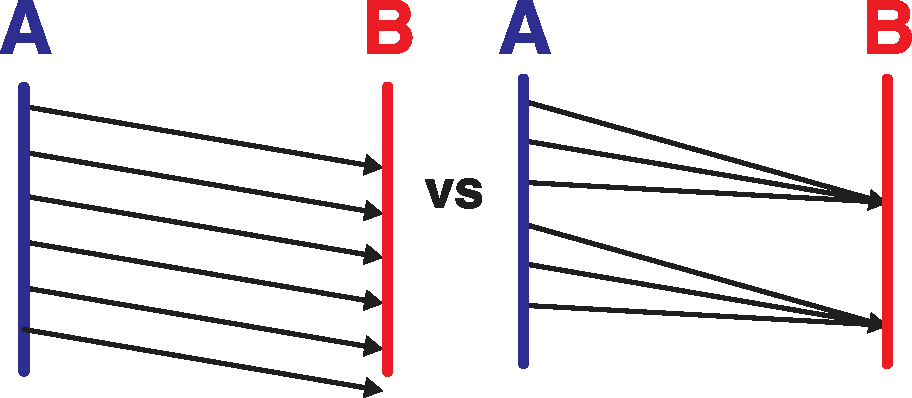
\includegraphics[width=\linewidth]{img/quality-of-service-metric-definitions/clumpiness.pdf}
    \caption{Clumpiness}
    \label{fig:quality-of-service-metric-definitions-clumpiness}
  \end{subfigure}%
  \begin{subfigure}[b]{0.5\textwidth}
    \centering
    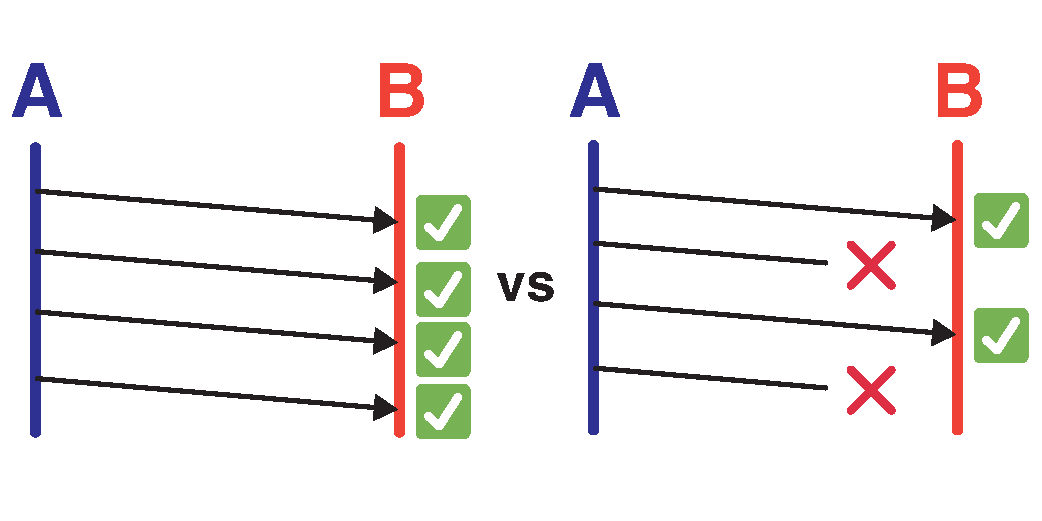
\includegraphics[width=\linewidth]{img/quality-of-service-metric-definitions/delivery-failure-rate.pdf}
    \caption{Delivery Failure Rate}
    \label{fig:quality-of-service-metric-definitions-delivery-failure-rate}
  \end{subfigure}
  \begin{subfigure}[b]{0.5\textwidth}
    \centering
    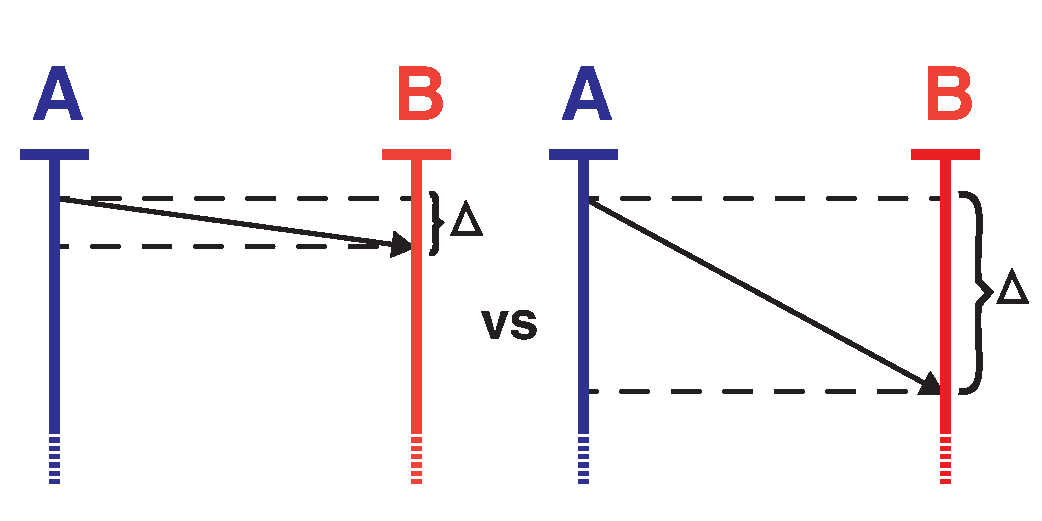
\includegraphics[width=\linewidth]{img/quality-of-service-metric-definitions/latency.pdf}
    \caption{Latency}
    \label{fig:quality-of-service-metric-definitions-latency}
  \end{subfigure}%
  \begin{subfigure}[b]{0.5\textwidth}
    \centering
    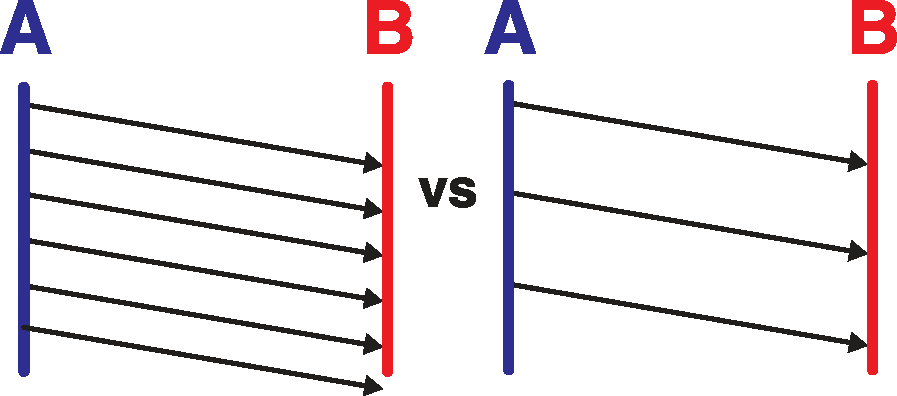
\includegraphics[width=\linewidth]{img/quality-of-service-metric-definitions/simstep-period.pdf}
    \caption{Simstep Period}
    \label{fig:quality-of-service-metric-definitions-simstep-period}
  \end{subfigure}%
  \caption{
  Quality of service metrics.
  Each illustration is a space-time diagram, with $A$ and $B$ representing independent processes.
  The vertical axis depicts the passage of time, from top to bottom.
  Solid black arrows represent message delivery.
  The left panel of each metric's diagram depicts a scenario with a lower (``better'') value for that metric compared to the right panel, which depicts a higher (``worse'') value for that metric.
  }
  \label{fig:quality-of-service-metric-definitions}
\end{figure*}


The best-effort communication model eschews effort to insulate of computation from real-time message delivery dynamics.
Because these dynamics are difficult to predict \textit{a priori} and can bias computation, thorough, empirical runtime measurements are necessary to understand results of such computation.
To this end, we developed a suite of quality of service metrics.
Figure \ref{fig:quality-of-service-metric-definitions} provides space-time diagrams illustrating the metrics presented in this section.

For the purposes of these metrics, we assume that simulations proceed in an iterative fashion with alternating compute and communication phases.
For short, we refer to a single compute-communication cycle as a ``simstep.''
We derive formulas for metrics in terms of independent observations preceding and succeeding a ``snapshot'' window, during which the simulation and any associated best-effort communication proceeds unimpeded.
Snapshot observations are taken at one minute intervals over the course of each of our a replicate experiments.
The following section, \ref{sec:quality-of-service-experiments}, details the experimental apparatus used to generate quality of service metrics reported in this work.

\subsubsection{Simstep Period} \label{sec:simstep-period-metric}

We calculate the amount of wall-time elapsed per simulation update cycle (``Simstep Period'') during a snapshot window as
\begin{align*}
\frac{
  \mathrm{update\,count\,after} - \mathrm{update\,count\,before}
}{
  \mathrm{walltime\,after} - \mathrm{walltime\,before}
}.
\end{align*}
Figure \ref{fig:quality-of-service-metric-definitions-simstep-period} compares a scenario with low simstep period to a scenario with a higher simstep period.

\subsubsection{Simstep Latency} \label{sec:wall-time-latency-metric}

This metric reports the number of simulation iterations that elapse between message dispatch and message delivery.
Figure \ref{fig:quality-of-service-metric-definitions-latency} compares a scenario with low latency to a scenario with a higher latency.

To insulate against imperfect clock synchronization between processes, we estimate one-way wall-time latency from a round-trip measure.
As part of our instrumentation, each simulation element maintains an independent zero-initialized ``touch counter'' associated with every neighbor simulation element it communicates with.
Dispatched messages originating from each simulation element are bundled with the value of the unique touch counter associated with the target element's counter.
When a message is received back to the originating element from the target element, the touch counter is set to $1 + \mathrm{bundled\,touch\,count}$.
In this manner, the touch counter increments by two for each successful round trip completed.
(Because simulation elements are arranged as a toroidal mesh, all interaction between simulation elements is reciprocal.)

We therefore calculate one-way latency during a snapshot window as,
\begin{align*}
  \frac{
    \mathrm{update\,count\,after} - \mathrm{update\,count\,before}
  }{
    \min\Big( \mathrm{ touch\,count\,after } - \mathrm{ touch\,count\,before }, 1 \Big)
  }.
\end{align*}
Note that if no touches elapsed during the snapshot window, we make a best-case assumption that one might elapse immediately after the end of the snapshot window (i.e., we count at least one elapsed touch).

%TODO reference @rodsan's derivation and proof

\subsubsection{Wall-time Latency} \label{sec:simulation-time-latency-metric}

Wall-time latency is closely related to simstep latency, except that interpret time in terms of elapsed simulation updates instead of wall time.
To calculate wall-time latency we apply a conversion to simstep latency based on simstep period,
\begin{align*}
  \mathrm{simstep\,latency} \times \mathrm{simstep\,period}.
\end{align*}

This metric directly tells the real-time performance of message transmission.
Although it directly follows from the interaction between simstep period and wall-time latency, it complements simstep latency's convenient interpretation in terms of potential simulation mechanics (e.g., simulation elements tending to see data from two updates ago versus from ten).

In addition to simstep latency, Figure \ref{fig:quality-of-service-metric-definitions-latency} is also representative of wall-time latency --- the difference being interpretation of $y$ axis in terms of wall-time instead of elapsed simulation updates.

\subsubsection{Delivery Failure Rate} \label{sec:delivery-failure-rate-metric}

Delivery failure rate measures the fraction of messages sent that are dropped.
The only condition where messages are dropped is when a send buffer fills.
(Under the existing MPI-based implementation, messages that queue on the send buffer are guaranteed for delivery.)
So, we can calculate
\begin{align*}
  \frac{
    \mathrm{successful\,send\,count\,after} - \mathrm{successful\,send\,count\,before}
  }{
    \mathrm{attempted\,send\,count\,after} - \mathrm{attempted\,send\,count\,before}
  }.
\end{align*}

\subsubsection{Delivery Clumpiness} \label{sec:delivery-clumpiness-metric}

Delivery clumpiness seeks to quantify the extent to which message arrival is consolidated to a subset of message pull attempts.
That is, the extent to which independently dispatched messages arrive in bundles rather than as an even stream.

If messages all arrive in independent pull attempts, then clumpiness will be zero.
At the point where the pigeonhole principle applies ($\mathrm{num\,arriving\,messages} >= \mathrm{num\,pull\,attempts}$), clumpiness will also be zero so long as every pull attempt is laden.
If all messages arrive during a single pull attempt, then clumpiness will approach 1.

We formulate clumpiness as the compliment of steadiness.
(Reporting clumpiness provides a lower-is-better interpretation consistent with the rest of the quality of service metrics.)
Steadiness, in turn, stems from three component statistics,
\begin{align*}
\mathrm{num\,laden\,pulls\,elapsed} =& \mathrm{laden\,pull\,count\,after} \\
  &- \mathrm{laden\,pull\,count\,before} \\
\mathrm{num\,messages\,received} =& \mathrm{message\,count\,after} \\
  &- \mathrm{message\,count\,before} \\
\mathrm{num\,pulls\,attempted} =& \mathrm{pull\,attempt\,count\,after} \\
  &- \mathrm{pull\,attempt\,count\,before}
.
\end{align*}

Here, we refer to pull attempts that successfully retrieve a message as ``laden.''

We combine $\mathrm{num\,messages\,received}$ and $\mathrm{num\,pulls\,attempted}$ to derive,
\begin{align*}
  \mathrm{num\,opportunities\,for\,laden\,pulls} = \\
   \min\Big(\mathrm{num\,messages\,received}, \mathrm{num\,pulls\,attempted}\Big).
\end{align*}

Then, to calculate steadiness,
\begin{align*}
  \frac{
    \mathrm{num\,laden\,pulls\,elapsed}
  }{
    \mathrm{num\,opportunities\,for\,laden\,pulls}
  }.
\end{align*}

Finally, we find delivery clumpiness as $1 - \mathrm{steadiness}$.
Figure \ref{fig:quality-of-service-metric-definitions-clumpiness} compares a scenario with low clumpiness to a scenario with higher clumpiness.


\subsection{Quality of Service Experiments} \label{sec:quality-of-service-experiments}

Quality of service experiments executed the graph coloring algorithm described in Section \ref{sec:graph-coloring-benchmark}.
In order to maximize communication intensity, only one graph vertex was assigned per cpu.

Quality of service experiments were carried out on Michigan State University's High Performance Computing Center lac cluster, consisting of 28-core Intel(R) Xeon(R) CPU E5-2680 v4 \@ 2.40GHz nodes.
Ten experimental replicates were performed for each condition surveyed.
Slightly over five minutes of runtime was afforded to each replicate.
Over five minutes of runtime, snapshots were taken at one minute intervals.
The first snapshot was taken one minute after the beginning of runtime.

Snapshots lasted one second, with the graph coloring algorithm running fully unhampered during the entire snapshot.
This was accomplished by collecting and recording data via a separate thread.
That thread collected and recorded a first tranche of snapshot data, spin waited for one second, and then recorded a second tranche.
Because of underlying system being observed shifts during data collection (somewhat akin to photographic motion blur), some intuitive invariants --- like strictly non-negative delivery failure rates --- do not hold in some cases.
However, the magnitude of such violations is generally minor.
Further, because data collection procedures were consistent across treatments, statistical comparisons between treatments remain sound, even if direct interpretation of reported metrics should be taken with a grain of salt.

Snapshots were performed independently for each process at each timepoint.
So, for example, for two processes over the five minute window of a single replicate ten snapshots were collected.
For statistical tests comparing treatments, snapshots were aggregated by replicate by either mean or median, as appropriate.
For each quality of service statistic we estimate mean --- which captures effects of extreme-magnitude outliers --- and median --- which more closely represents typicalness --- across these window samples.
Statistical comparisons across treatment conditions are performed via regression.
We use ordinary least squares regression to analyze means \cite{geladi1986partial} and quantile regression to analyze medians \cite{koenker2001quantile}.
For comparisons between dichotomous, categorical treatment conditions, one condition is coded as 0 and the other as 1.
In the case of ordinary least squares regression, this boils down to an independent $t$-test.
Although quantile regression on categorical predictors is not precisely equivalent to a direct test on medians between two groups (i.e., Mood's median test), there is precedent for this approach \cite{petscher2014quantile, konstantopoulos2019using}.

Most statistics reported here can be calculated just as well in terms of incoming or outgoing messages.
That is, most statistics can be generated via data from instrumentation attached to message ``inlets'' or data from instrumentation attached to message ``outlets'' with no obvious reason to prefer one over the other.
Although ``inlet-'' and ``outlet-''derived statistics are nearly identical in all cases, for completeness we include both.


\subsection{Code, Data, and Reproducibility}

\subsubsection{Benchmarking Experiments} \label{sec:methods-code-data-reproducibility-benchmarking-experiments}

Benchmarking experiments were performed on Michigan State University's High Performance Computing Center, a cluster of hundreds of heterogeneous x86 nodes linked with InfiniBand interconnects.
For multithread experiments, benchmarks for each thread count were collected from the same node.
For multiprocess experiments, each processes was assigned to a distinct node in order to ensure results were representative of performance in a distributed context.
All multiprocess benchmarks were recorded from the same collection of nodes.
Hostnames are recorded for each benchmark data point.
For an exact accounting of hardware architectures used, these hostnames can be crossreferenced with a table included with the data that summarizes the cluster's node configurations.

Code for the distributed graph coloring benchmark is available at \url{https://github.com/mmore500/conduit} under \\ \texttt{demos/channel\_selection}.
Code for the digital evolution simulation benchmark is available at \url{https://github.com/mmore500/dishtiny}.
Exact versions of software used are recorded with each benchmark data point.
Data is available via the Open Science Framework at \url{https://osf.io/7jkgp/} \citep{foster2017open}.
A live, in-browser notebook for all reported statistics and data visualizations and is available via Binder at \url{https://mybinder.org/v2/gh/mmore500/conduit/binder?filepath=binder%2Fdate%3D2021%2Bproject%3D7jkgp} \citep{jupyter2018binder}.

\subsubsection{Quality of Service Experiments}

Quality of service experiments were performed on Quality of service experiments were carried out on Michigan State University's High Performance Computing Center lac cluster, consisting of 28-core Intel(R) Xeon(R) CPU E5-2680 v4 \@ 2.40GHz nodes.
All statistical comparisons are performed between observations from the same job allocation.
(Except in the case where intranode and internode configurations were compared, where experiments were performed on separate allocations using comparable nodes on the same cluster.)

Benchmarking experiments described in Section \ref{sec:methods-code-data-reproducibility-benchmarking-experiments} used a send/receive buffer size of 2.
However, due to the high communication intensity of the graph coloring problem with just one simulation element per CPU, quality of service experiments required a larger buffer size of 64 to maintain runtime stability.
In early work developing the Conduit library, we discovered that real-time messaging channels can enter a destabilizing positive feedback spiral when incoming messages take longer to handle (e.g., skip past or read) than sending messages.
Under such conditions, when a process exchanging messages from a partner process experiences a delay it sends fewer messages to that partner process.
Due to fewer incoming messages, the partner the partner process can update more rapidly, increasing incoming message load on the delayed process.
This effect can snowball the partnership intended for even, two-way message exchange into effectively a unilateral producer-consumer relationship where (potentially unbounded) work piles up on the consumer.
To interrupt such a scenario, we use the bulk message pull call \verb|MPI_Testsome| to ensure fast message consumption under backlogged conditions.
So, receiver workload remains closer to constant under high traffic situations (instead of having to pull messages down one-by-one).
Larger receive buffer size, as configured for the quality of service experiments, increases the effectiveness of the bulk message consumption countermeasure.

Code for the distributed graph coloring benchmark is available at \url{https://github.com/mmore500/conduit} under \\ \texttt{demos/channel\_selection}.
Exact versions of software used are recorded with each benchmark data point.
Data is available via the Open Science Framework at \url{https://osf.io/72k5n/} \citep{foster2017open}.
A live, in-browser notebook for all reported statistics and data visualizations is available via Binder at \url{https://mybinder.org/v2/gh/mmore500/conduit/binder?filepath=binder%2Fdate%3D2021%2Bproject%3D72k5n} \citep{jupyter2018binder}.

